
%(BEGIN_QUESTION)
% Copyright 2004, Tony R. Kuphaldt, released under the Creative Commons Attribution License (v 1.0)
% This means you may do almost anything with this work of mine, so long as you give me proper credit

Calculate the source current and load current in this transformer circuit:

$$\includegraphics[width=15.5cm]{i04757x01.eps}$$

$I_{source}$ = \hskip 80pt $I_{load}$ =

\vskip 20pt \vbox{\hrule \hbox{\strut \vrule{} {\bf Suggestions for Socratic discussion} \vrule} \hrule}

\begin{itemize}
\item{} Identify which fundamental principles of electric circuits apply to each step of your analysis of this circuit.  In other words, be prepared to explain the reason(s) ``why'' for every step of your analysis, rather than merely describing those steps.
\item{} Would this transformer be referred to as a {\it step-up} or a {\it step-down}, and why?
\item{} Can a step-down transformer be used as a step-up, and vice-versa?  Why or why not?
\end{itemize}

\underbar{file i04757}
%(END_QUESTION)





%(BEGIN_ANSWER)

$I_{source}$ = 187.5 mA \hskip 80pt $I_{load}$ = 72.73 mA

%(END_ANSWER)





%(BEGIN_NOTES)

Transformer step-up ratio = ${3610 \over 1400}$ = 2.5786:1.

\vskip 10pt

$V_{sec} = (110)(2.5786) = 283.64$ volts

\vskip 10pt

$I_{load} = {283.64 \over 3900}$ = 72.73 mA

\vskip 10pt

$I_{pri} = (72.73 \hbox{ mA})(2.5786) = 187.54$ mA

%INDEX% Electronics review: AC transformer circuit

%(END_NOTES)


